% !TEX encoding = UTF-8
% !TEX TS-program = pdflatex
% !TEX root = ../tesi.tex

%**************************************************************
\chapter{Introduction}\label{ch:introduction}
%**************************************************************

\intro{In this section we will present the summarized content of the whole thesis.}
%\noindent Esempio di utilizzo di un termine nel glossario \\
%\gls{api}. \\
%
%\noindent Esempio di citazione in linea \\
%\cite{site:agile-manifesto}. \\
%
%\noindent Esempio di citazione nel pie' di pagina \\
%citazione\footcite{womak:lean-thinking} \\

%**************************************************************

\section{Background}\label{sec:background}
Computer vision (CV) is a field of artificial intelligence that deals with the study of how computers can be made to gain high-level understanding from digital images or videos.
If AI allows the computer to think like a human as well as computer vision allows the computer to see like a human.

CV works like the human visual system, with the big difference in the fact that human uses year and year of experience to help the mind to understand what it is seeing.
As the biological neurons processes the information in the brain, the artificial neurons processes the information in the artificial neural network following the Hebbian plasticity (\cite{site:hebbian-plasticity}) rule: the connection between two neurons is strengthened if they are active at the same time.

In recent years, deep learning has revolutionized the CV field, achieving excellent results in many tasks, like: image classification, object detection, semantic segmentation, image captioning, image generation, etc.

The image classification task consists of assigning a label to an image with only one object (\hyperref[fig:figure-tulips]{Figure 1.1}).
\begin{figure}[H]
    \centering
    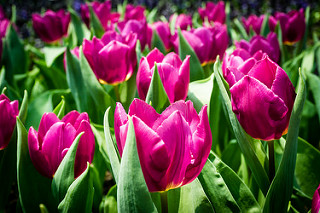
\includegraphics[width=0.8\textwidth]{images/1_1_tulips}
    \caption[Example of image classification]{Image classification: this image is classified as a tulip}
    \label{fig:figure-tulips}
\end{figure}
The object detection tasks consists of assigning a label and a bounding box to each object in the image.
The bounding box is a rectangle that encloses the object(\hyperref[fig:figure-object-detection]{Figure 1.2}).
\begin{figure}[H]
    \centering
    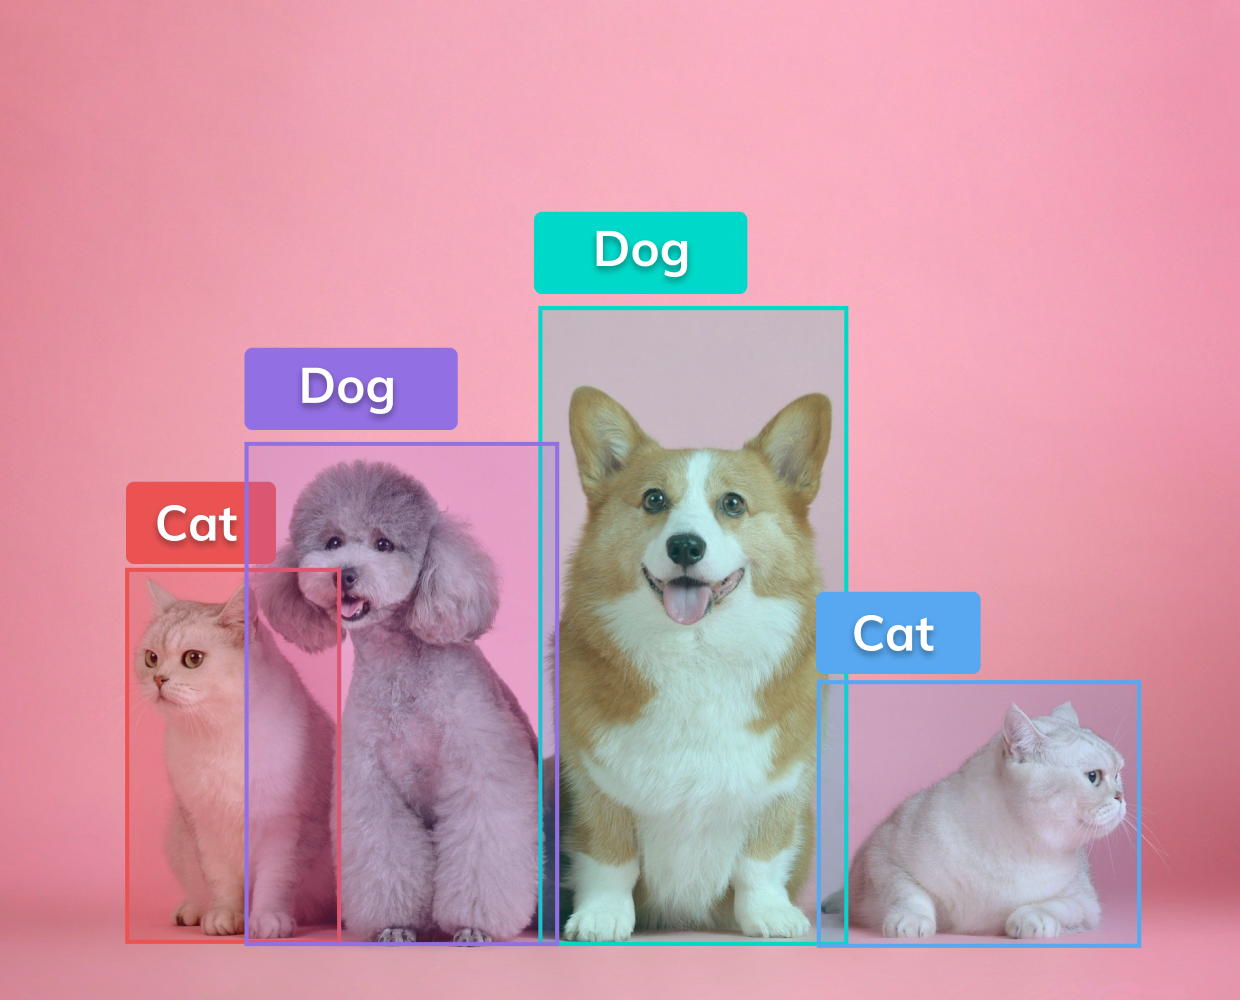
\includegraphics[width=0.8\textwidth]{images/1_1_object_detection}
    \caption[Example of object detection]{Object detection: this image contains two classes of objects, cat and dog.}
    \label{fig:figure-object-detection}
\end{figure}
The semantic segmentation task consists of assigning a label to each pixel of the image(\hyperref[fig:figure-semantic-segmentation]{Figure 1.3}).

\begin{figure}[H]
    \centering
    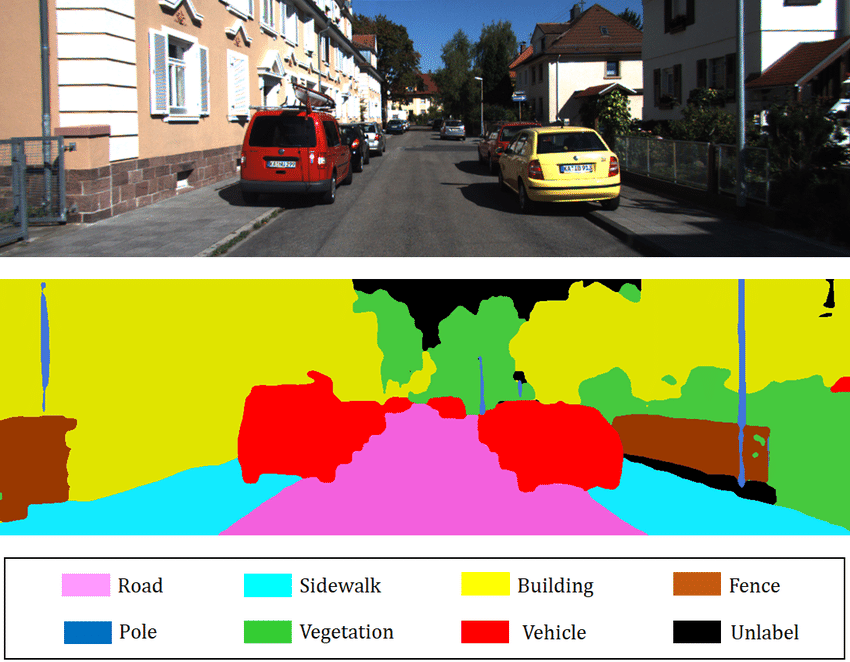
\includegraphics[width=0.8\textwidth]{images/1_1_semantic_segmentation}
    \caption[Example of semantic segmentation]{Semantic segmentation: each pixel is assigned a label.}
    \label{fig:figure-semantic-segmentation}
\end{figure}

Then, the modern CV systems can be used not only on the images, but also on video, like surveillance cameras to perform the real-time object detection and tracking, the most famous model is YOLOv3 (Redmon et al.~\cite{yolov3_paper}) (\hyperref[fig:figure-yolo-v3]{Figure 1.4}).

\begin{figure}[H]
    \centering
    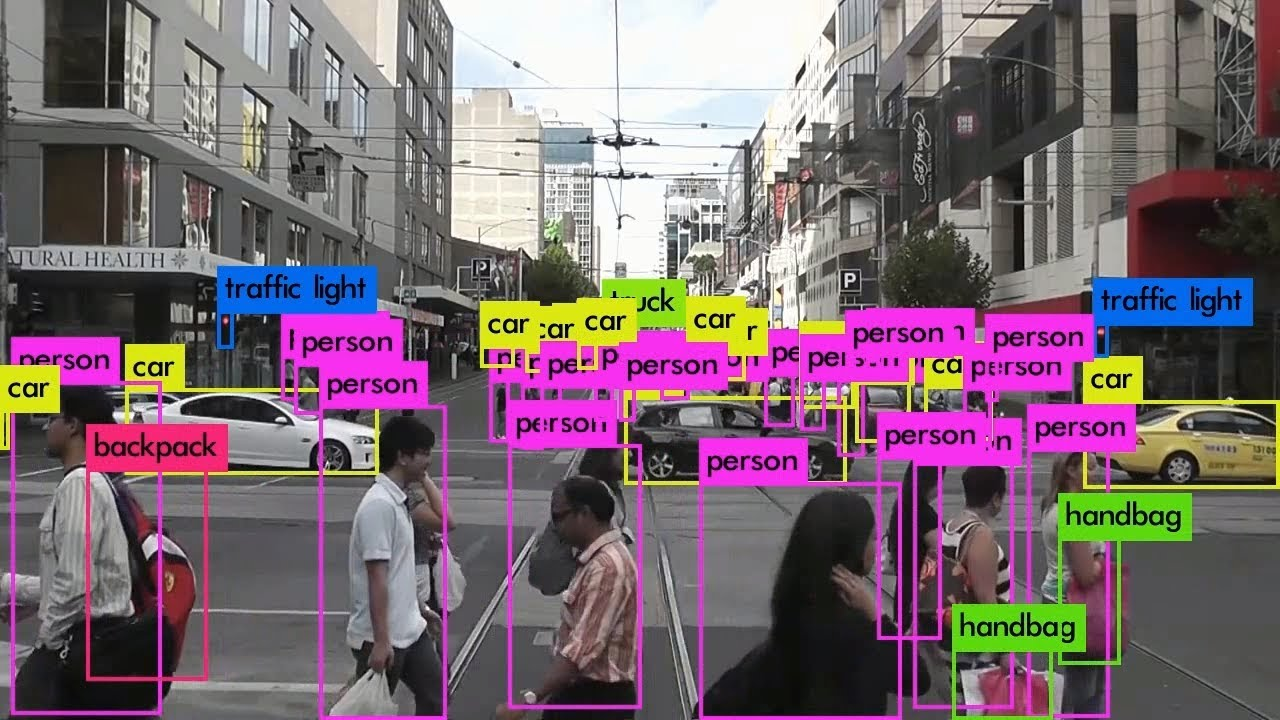
\includegraphics[width=0.8\textwidth]{images/1_1_yolov3}
    \caption{YOLO-V3 in action.}
    \label{fig:figure-yolo-v3}
\end{figure}



%**************************************************************

\section{Problem}\label{sec:problem}
The term "odometry" originated from two Greek works \emph{hodos} (meaning "journery" or "travel") and \emph{metron} (meaning "measure").
This derivation is related to the estimation of the change in a robot's pose (translation and rotation) over time.
Mobile robot use data from motion sensor to estimate their position relative to their initial location, this is called odometry.
VO is a technique used to localize a robot by using only a stream of images acquired from a single or multiple camera.
There are different ways to classify the typology of Visual Odometry:
\begin{itemize}
    \item based on the camera setup:
        \begin{itemize}
            \item Monocular VO: using only one camera;
            \item Stereo VO: using two cameras;
        \end{itemize}
    \item based on the information:
        \begin{itemize}
            \item Feature based method: which extracts the image feature points and tracks them in the image sequence;
            \item Direct method: a novel method which uses the pixel intensity in the image sequence directly as visual input.
            \item Hybrid method: which combines the two methods.
        \end{itemize}
    \item Visual inertial odometry: if a \gls{imu} is used within the VO system, it is commonly referred to as Visual inertial odometry.
\end{itemize}
We can represent the pose in different ways, for example: \textbf{euler angles}, \textbf{quaternions}, \textbf{rotation matrices} combined with \textbf{translation vectors}.

The goal is to create a \gls{nn}, using a \textbf{ResNet} to extract features from images and the \textbf{transformer} presented by Vaswani et al.~(\cite{transformer_paper}), which is able to estimate a sequence of camera poses given a sequence of images.

%**************************************************************

\section{Why transformer?}\label{sec:why-transformer}

We think that the transformer is a good candidate to solve the problem of visual odometry because it is able to learn a sequence from one domain and translate it into another sequence from another domain.
This kind of task is called sequence-to-sequence translation, e.g., machine translation.

Traditionally, this task is tackled by using recurrent neural networks (RNNs), but they have some limitations, such as the vanishing gradient problem, which makes them difficult to train.

Other VO approaches uses the CNNs, but in CNNs the features are statically weighted using pretrained weights, while in the transformer the features are dynamically weighted based on the context and receptive fields of CNNs can be limiting the performance of the whole network.
The success of the CNN derives from the fact the shared weights explicitly encode how specific identical patterns are repeated in images, this ensures the convergence also in relatively small dataset, but also limits the modelling capacity.
Meaning that CNNs can converge to a good performance also with a relatively small dataset.

Meanwhile, the vision transformers do not enforce such strict bias, so, transformer has the higher learning capacity, but it's harder to train.

So, given the high learning capacity of the transformer, its capability to adapt to various tasks and its good ability in seq2seq translation, we think that it is a good candidate to solve the problem of visual odometry.


%**************************************************************


\section{Solution}\label{sec:solution}
%**************************************************************
Researchers proposed special adversarial attacks in the text domain in order to maintain semantic consistency and syntactic correctness.
But those methods fail in generating high-quality adversarial examples since they frequently violate linguistic constraints.

This thesis concentrates on the adversarial attacks for text classification, in particular, the attacks based on sentiment analysis datasets, like IMDB \cite{maas-EtAl:2011:ACL-HLT2011} and Rotten Tomatoes \cite{pang-lee:2005a}.
Two state-of-the-art approaches, TextFooler \cite{journals/corr/abs-1907-11932} and BERT-based attack \cite{conf/emnlp/GargR20}, are compared to analyze weaknesses and strengths.

Then, their shortcomings are addressed by proposing a novel method, called SynBA, to generate adversarial examples for text data.
It is a word-level attack that generates adversarial examples by substituting words with candidates that have both a synonymy and contextual relationship with the original token.

The key contributions of this survey can be summarized as follows:
\begin{itemize}
    \item we introduce a simple but strong attack method, SynBA, to quickly generate high-profile utility-preserving adversarial examples that force the target models to make wrong predictions under the white-box setting;
    \item we propose a comprehensive automatic and human evaluation of adversarial attacks to evaluate the effectiveness, efficiency, and utility preserving properties of our system;
    \item we compare the adversarial examples generated by our method with TextFooler and BERT-based attack in terms of semantic similarity, semantic consistency, perturbation rate, success rate, perplexity and execution time.
\end{itemize}


% Our contributions. This survey concentrates on the adversarial
% attack and defense technology in the NLP field and provides a thorough and systematic review. 
%The key contributions of this survey
% can be summarized as follows:
%  We comprehensively and systematically summarize the textual
% adversarial attack and defense technology, elaborating on textual adversarial examples, adversarial attacks on texts, defenses
% against textual adversarial attacks, applications in various NLP
% tasks, and potential development directions in this domain.
%  We categorize current textual adversarial attacks according to
% the semantic granularity at the top level and further classify
% each class into several subclasses depending on the example
% generation strategy. To the best of our knowledge, we are the
% first to regard the example generation strategy as a classification criterion and propose this two-level classification for
% adversarial attacks.

%

% Briefly describe your methodology and/or theoretical approach
% Explain the aim of your research and what contribution it will make to the topic

% from TextFooler

% Our main contributions are summarized as follows:
% • We propose a simple but strong baseline, TEXTFOOLER, to quickly generate high-profile utility-preserving adversarial examples that force the target models to make wrong predictions under the black-box setting.
% • We evaluate TEXTFOOLER on three state-of-the-art deep learning models over five popular text classification tasks and two textual entailment tasks, and it achieved the state-of-the-art attack success rate and perturbation rate. Algorithm 1 Adversarial Attack by TEXTFOOLER
% • We propose a comprehensive four-way automatic and three-way human evaluation of language adversarial attacks to evaluate the effectiveness, efficiency, and utilitypreserving properties of our system.
% • We open-source the code, pre-trained target models, and test samples for the convenience of future benchmarking


%**************************************************************

\section{Thesis organization}\label{sec:thesis-organization}
\begin{description}
    \item[{\hyperref[ch:introduction]{First chapter}}] introduces the general content about thesis and gives a short presentation of the topic, the problem and the solution we propose;

    \item[{\hyperref[ch:background]{Second chapter}}] a deepening about the theoretical foundations used during the stage and the project;

    \item[{\hyperref[ch:methodology]{Third chapter}}] presents the datasets used during for the training and the testing of the model;

    \item[{\hyperref[ch:experimental-results]{Fourth chapter}}] presents the experiments did during to develop the system;

    \item[{\hyperref[ch:final-discussions]{Fifth chapter}}] discusses about the results and possible future developments.
\end{description}
During the drafting of the essay, following typography conventions are considered:
\begin{itemize}
    \item the acronyms, abbreviations, ambiguous terms or terms not in common use are defined in the glossary, in the end of the present document;
    \item the first occurrences of the terms in the glossary are highlighted like this: \gls{word};
    \item the terms from the foreign language or jargon are highlighted like this: \emph{italics}.
\end{itemize}

%**************************************************************

